\documentclass[12pt, twoside]{article}
\input{../preamble}
\usepackage{pgfplots}
\pgfplotsset{compat=1.18}

\fancyhead[LE]{\thepage}
\fancyhead[RO]{Name: \hspace{4cm} \,\\ \hspace{2.9cm} \,}
\fancyhead[LO]{La Scuola d'Italia / Dr.\ Huson / IB Math \\* 27 March 2026}

\begin{document}
\subsubsection*{6.2 Classwork: Quadratics}

\begin{enumerate}[itemsep=0.2cm]

%--- Problem 1: Tangent line to parabola / discriminant (lecture problem) [10 marks] ---
\item The diagram below shows the parabola $y = x^2 - 2x$ and the line $y = 4x + k$,
where $k$ is a constant. The line is tangent to the parabola at the point $P$.

\begin{center}
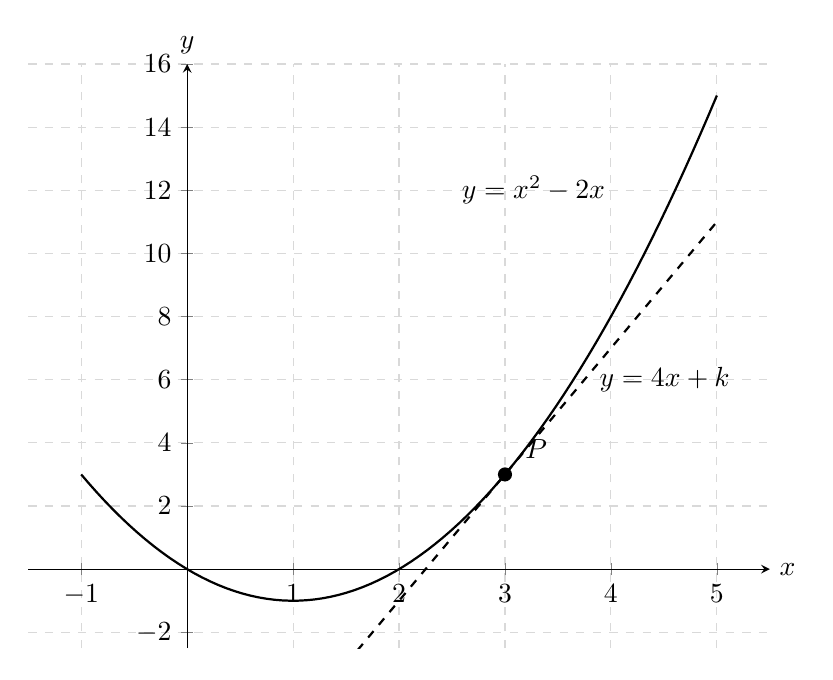
\begin{tikzpicture}
\begin{axis}[
  axis lines=middle,
  xlabel={$x$},
  ylabel={$y$},
  grid=both,
  grid style={dashed, gray!30},
  xmin=-1.5, xmax=5.5,
  ymin=-2.5, ymax=16,
  xtick={-1,0,...,5},
  ytick={-2,0,2,...,16},
  width=11cm,
  height=9cm,
  every axis x label/.style={at={(ticklabel* cs:1.0)}, anchor=west},
  every axis y label/.style={at={(ticklabel* cs:1.0)}, anchor=south},
]
  % Parabola
  \addplot[thick, domain=-1:5, samples=80] {x^2 - 2*x};
  % Tangent line
  \addplot[thick, dashed, domain=0.5:5] {4*x - 9};
  % Point of tangency
  \node[circle, fill, inner sep=1.8pt] at (axis cs:3,3) {};
  \node[anchor=south west] at (axis cs:3.1,3.2) {$P$};
  % Labels
  \node[anchor=west] at (axis cs:2.5,12) {$y = x^2 - 2x$};
  \node[anchor=west] at (axis cs:3.8,6) {$y = 4x + k$};
\end{axis}
\end{tikzpicture}
\end{center}

\begin{enumerate}[itemsep=0.15cm]
  \item Write down an equation whose solutions give the $x$-coordinates of
        the points where the line meets the parabola. \hfill [2]
  \item Simplify your equation to the form $x^2 + bx + c = 0$, stating $b$
        and $c$ in terms of $k$. \hfill [2]
  \item For the line to be tangent, state the condition on the discriminant. \hfill [1]
  \item Find the value of $k$. \hfill [3]
  \item Find the coordinates of the point $P$. \hfill [2]
\end{enumerate}

\newpage

%--- Problem 2: Vertex form and graph properties [8 marks] ---
\item Let $f(x) = -x^2 + 4x + 5$.

\begin{enumerate}[itemsep=0.15cm]
  \item Write $f(x)$ in the form $-(x - h)^2 + k$. \hfill [3]
  \item Write down the coordinates of the vertex of the parabola. \hfill [1]
  \item Write down the equation of the axis of symmetry. \hfill [1]
  \item Find the $x$-intercepts of the graph of $f$. \hfill [2]
  \item Write down the $y$-intercept. \hfill [1]
\end{enumerate}

\begin{tikzpicture}
  \draw (0,0) rectangle (15.5,11);
  \foreach \y in {1,2,...,10} \draw [dotted] (0.5,\y)--(15,\y);
\end{tikzpicture}

\newpage

%--- Problem 3: Discriminant and parameter conditions [8 marks] ---
\item The equation $2x^2 - 4x + p = 0$ has two distinct real roots, where $p \in \mathbb{R}$.

\begin{enumerate}[itemsep=0.15cm]
  \item Find the discriminant of the equation in terms of $p$. \hfill [2]
  \item Find the values of $p$ for which the equation has two distinct real roots. \hfill [2]
  \item Find the values of $p$ for which the equation has no real roots. \hfill [1]
  \item Find the value of $p$ for which there is exactly one real root,
        and find that root. \hfill [3]
\end{enumerate}

\begin{tikzpicture}
  \draw (0,0) rectangle (15.5,12);
  \foreach \y in {1,2,...,11} \draw [dotted] (0.5,\y)--(15,\y);
\end{tikzpicture}

\newpage

%--- Problem 4: Line and parabola intersection [9 marks] ---
\item The parabola $y = x^2 - 2x - 3$ and the line $y = x + 1$ are drawn
on the same axes.

\begin{enumerate}[itemsep=0.15cm]
  \item Show that the $x$-coordinates of the points of intersection satisfy\\
        $x^2 - 3x - 4 = 0$. \hfill [2]
  \item Factorise $x^2 - 3x - 4$. \hfill [1]
  \item Hence find the coordinates of the two points of intersection. \hfill [3]
  \item Find the equation of the axis of symmetry of the parabola. \hfill [1]
  \item Find the coordinates of the vertex of the parabola. \hfill [2]
\end{enumerate}

\begin{tikzpicture}
  \draw (0,0) rectangle (15.5,10);
  \foreach \y in {1,2,...,9} \draw [dotted] (0.5,\y)--(15,\y);
\end{tikzpicture}

\end{enumerate}
\end{document}

Solutions
  Problem 1 — Tangent to parabola via discriminant:
  - (a) x² - 2x = 4x + k
  - (b) x² - 6x - k = 0, so b = -6, c = -k
  - (c) Δ = 0 (exactly one solution)
  - (d) Δ = 36 + 4k = 0 → k = -9
  - (e) x² - 6x + 9 = 0 → (x-3)² = 0 → x = 3, y = 9 - 6 = 3. P = (3, 3)

  Problem 2 — Vertex form:
  - (a) f(x) = -(x² - 4x) + 5 = -(x² - 4x + 4) + 4 + 5 = -(x - 2)² + 9
  - (b) Vertex = (2, 9)
  - (c) x = 2
  - (d) -(x-2)² + 9 = 0 → (x-2)² = 9 → x = -1 or x = 5
  - (e) f(0) = 5, y-intercept = (0, 5)

  Problem 3 — Discriminant parameter:
  - (a) Δ = (-4)² - 4(2)(p) = 16 - 8p
  - (b) 16 - 8p > 0 → p < 2
  - (c) 16 - 8p < 0 → p > 2
  - (d) 16 - 8p = 0 → p = 2. Then 2x² - 4x + 2 = 0 → x² - 2x + 1 = 0 → (x-1)² = 0 → x = 1

  Problem 4 — Line and parabola:
  - (a) x² - 2x - 3 = x + 1 → x² - 3x - 4 = 0
  - (b) (x - 4)(x + 1) = 0
  - (c) x = 4, y = 5 → (4, 5); x = -1, y = 0 → (-1, 0)
  - (d) x = -b/(2a) = 3/2 = 1. Wait: axis of symmetry of x² - 2x - 3 is x = -(-2)/(2·1) = 1
  - (e) f(1) = 1 - 2 - 3 = -4. Vertex = (1, -4)
